\begin{frame}{Marking season}
	\begin{columns}
		\begin{column}{0.47\textwidth}
			\includegraphics[width=\textwidth]{libraryPapers3} \pause
		\end{column}
		\begin{column}{0.47\textwidth}
			\begin{itemize}
				\item A course has $n$ students \pause
				\item Each student hands in an essay \pause
				\item The administration sets the markers a number of tasks...
			\end{itemize}
		\end{column}
	\end{columns}
\end{frame}

\begin{frame}{Task 1: mark the work}
	Socrative room code: \texttt{FALCOMPED}
	\begin{itemize}
		\item It takes \textbf{1 hour} to mark \textbf{1 essay} \pause
		\item If $n=10$, how long does marking take? \pause
		\item If $n=20$, how long does marking take? \pause
		\item If the number of students \textbf{doubles}, what happens to the time marking takes?
	\end{itemize}
\end{frame}

\begin{frame}{Linear time}
	\begin{columns}
		\begin{column}{0.47\textwidth}
			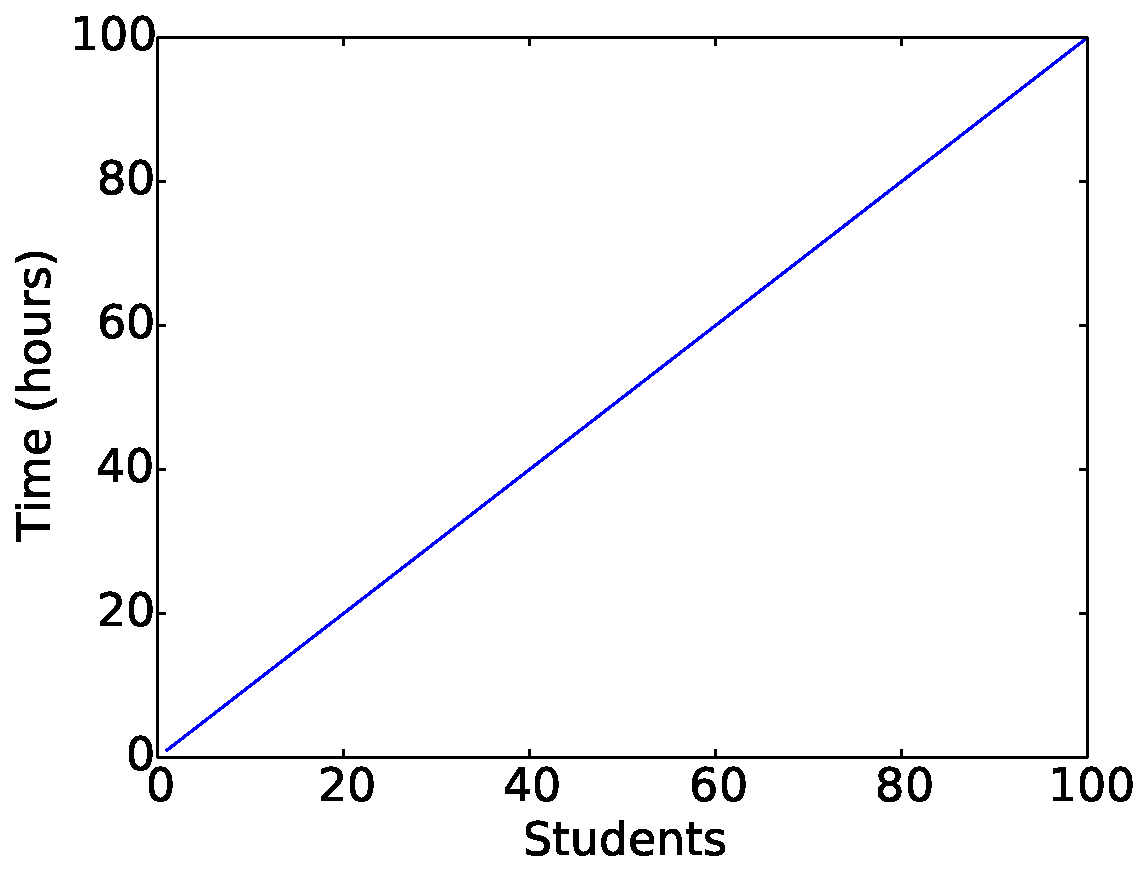
\includegraphics[width=\textwidth]{plot_linear}
		\end{column}
		\begin{column}{0.47\textwidth}
			\begin{itemize}
				\item Marking the work is a \textbf{linear time operation} \pause
				\item \textbf{Doubling} the number of students \textbf{doubles} the time it takes \pause
				\item Notation: the time complexity of this task is $O(n)$ \pause
				\begin{itemize}
					\item Meaning: the time it takes is roughly $c \times n$, for some constant $c$
				\end{itemize}
			\end{itemize}
		\end{column}
	\end{columns}
\end{frame}

\begin{frame}{Task 2: weigh the work}
	Socrative room code: \texttt{FALCOMPED}
	\begin{itemize}
		\item It takes \textbf{5 hours} to calibrate the scales,
			load the stack of essays (\textbf{no matter how large}) and take a reading \pause
		\item If $n=10$, how long does weighing take? \pause
		\item If $n=20$, how long does weighing take? \pause
		\item If the number of students \textbf{doubles}, what happens to the time it takes?
	\end{itemize}
\end{frame}

\begin{frame}{Constant time}
	\begin{columns}
		\begin{column}{0.47\textwidth}
			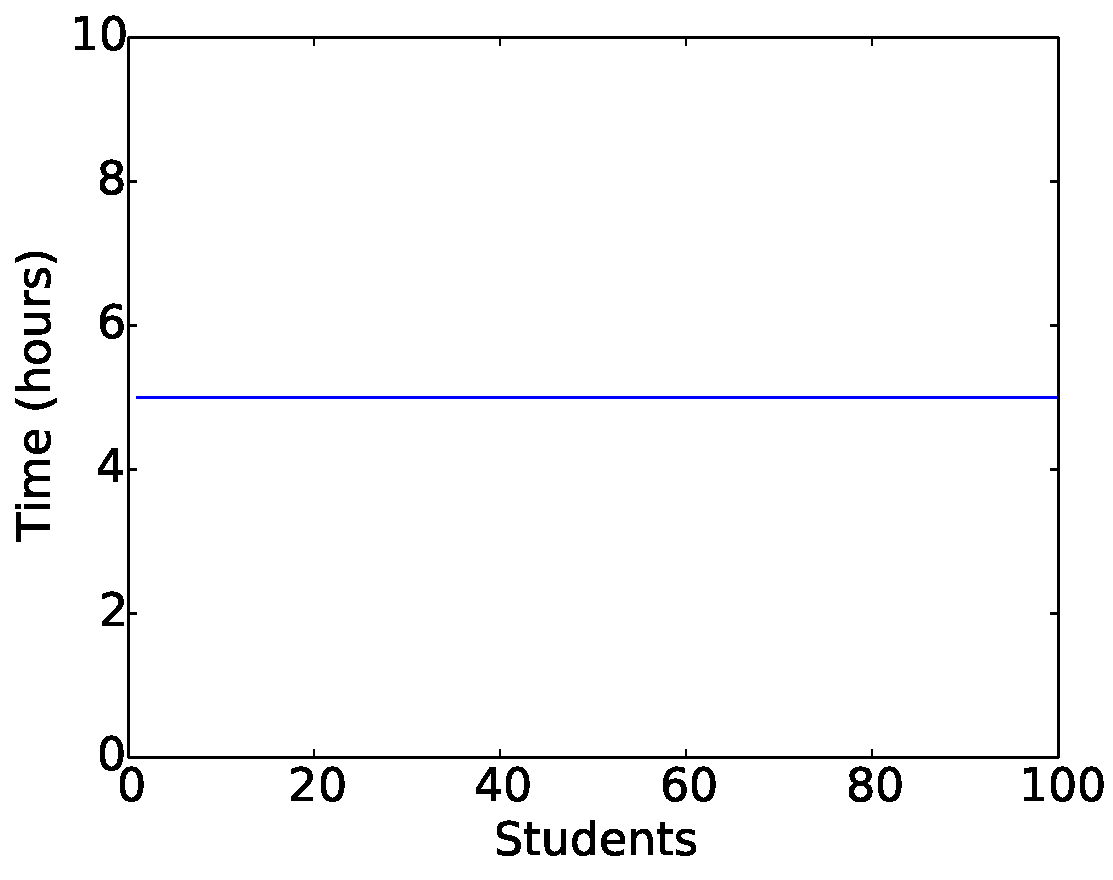
\includegraphics[width=\textwidth]{plot_constant}
		\end{column}
		\begin{column}{0.47\textwidth}
			\begin{itemize}
				\item Weighing the work is a \textbf{constant time operation} \pause
				\item \textbf{Doubling} the number of students \textbf{does not change} the time it takes \pause
				\item Notation: the time complexity of this task is $O(1)$ \pause
				\begin{itemize}
					\item Meaning: the time it takes is roughly $c$, for some constant $c$
				\end{itemize}
			\end{itemize}
		\end{column}
	\end{columns}
\end{frame}

\begin{frame}{Task 3: check for plagiarism}
	Socrative room code: \texttt{FALCOMPED}
	\begin{itemize}
		\item It takes \textbf{10 minutes} to check \textbf{a pair} of essays for plagiarism \pause
		\item How many pairs are there? \pause
		\begin{itemize}
			\item $(n-1) + (n-2) + (n-3) + \dots + 2 + 1$ \pause
			\item $= \frac12 \times n \times (n-1)$ \pause
		\end{itemize}
		\item If $n=10$, how long does checking take?
		\begin{itemize}
			\item Hint: there are $\frac12 \times \left( 10^2 - 10 \right) = 45$ pairs \pause
		\end{itemize}
		\item If $n=20$, how long does checking take?
		\begin{itemize}
			\item Hint: there are $\frac12 \times \left( 20^2 - 20 \right) = 190$ pairs \pause
		\end{itemize}
		\item If the number of students \textbf{doubles}, what happens to the time it takes?
	\end{itemize}
\end{frame}

\begin{frame}{Quadratic time}
	\begin{itemize}
		\item The time it takes is $10 \times \frac12 \times n \times (n-1)$ \pause
		\item If $n$ is large, $n \times (n-1) \approx n^2$ \pause
		\item So the time it takes is roughly $c \times n^2$ for some constant $c$ ($10 \times \frac12$ in this case)
	\end{itemize}
\end{frame}

\begin{frame}{Quadratic time}
	\begin{columns}
		\begin{column}{0.47\textwidth}
			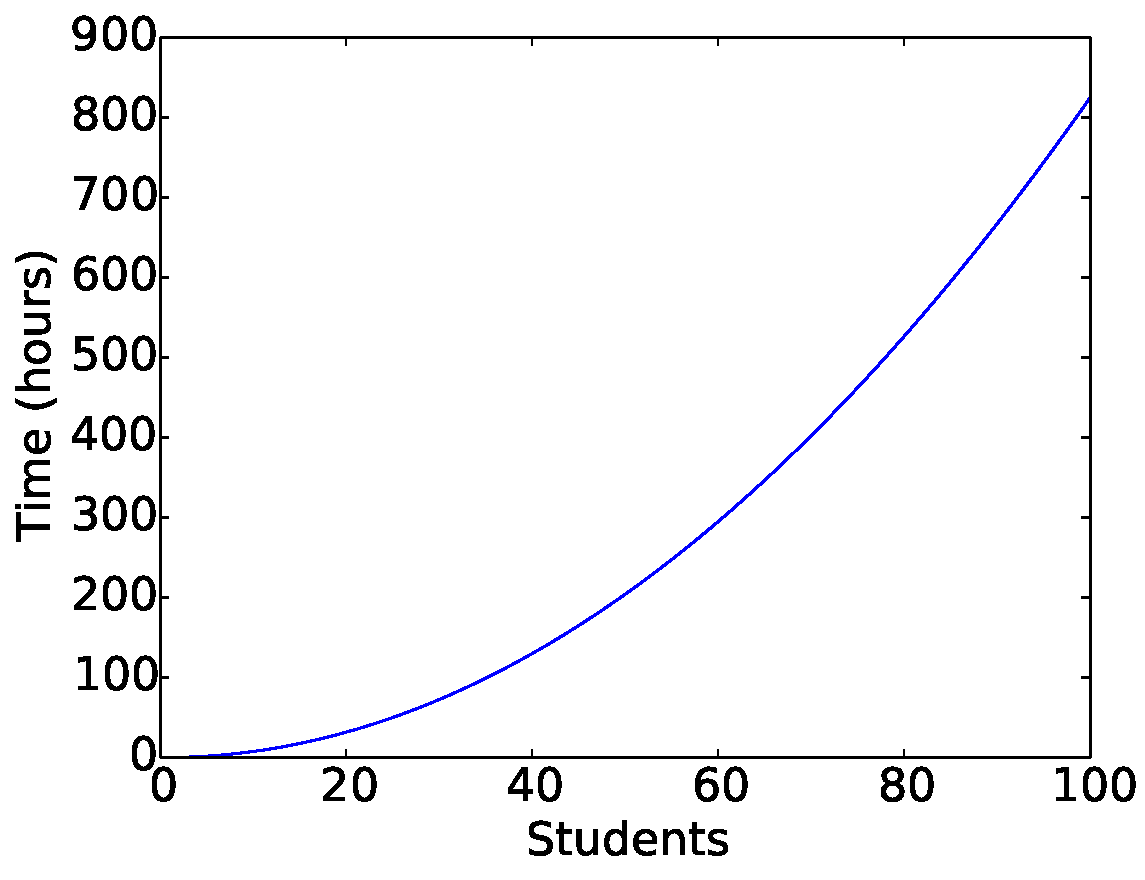
\includegraphics[width=\textwidth]{plot_quadratic}
		\end{column}
		\begin{column}{0.47\textwidth}
			\begin{itemize}
				\item Weighing the work is a \textbf{quadratic time operation} \pause
				\item \textbf{Doubling} the number of students \textbf{quadruples} the time it takes \pause
				\item Notation: the time complexity of this task is $O(n^2)$ \pause
				\begin{itemize}
					\item Meaning: the time it takes is roughly $c \times n^2$, for some constant $c$
				\end{itemize}
			\end{itemize}
		\end{column}
	\end{columns}
\end{frame}

\begin{frame}{Recap}
	\begin{columns}
		\begin{column}{0.47\textwidth}
			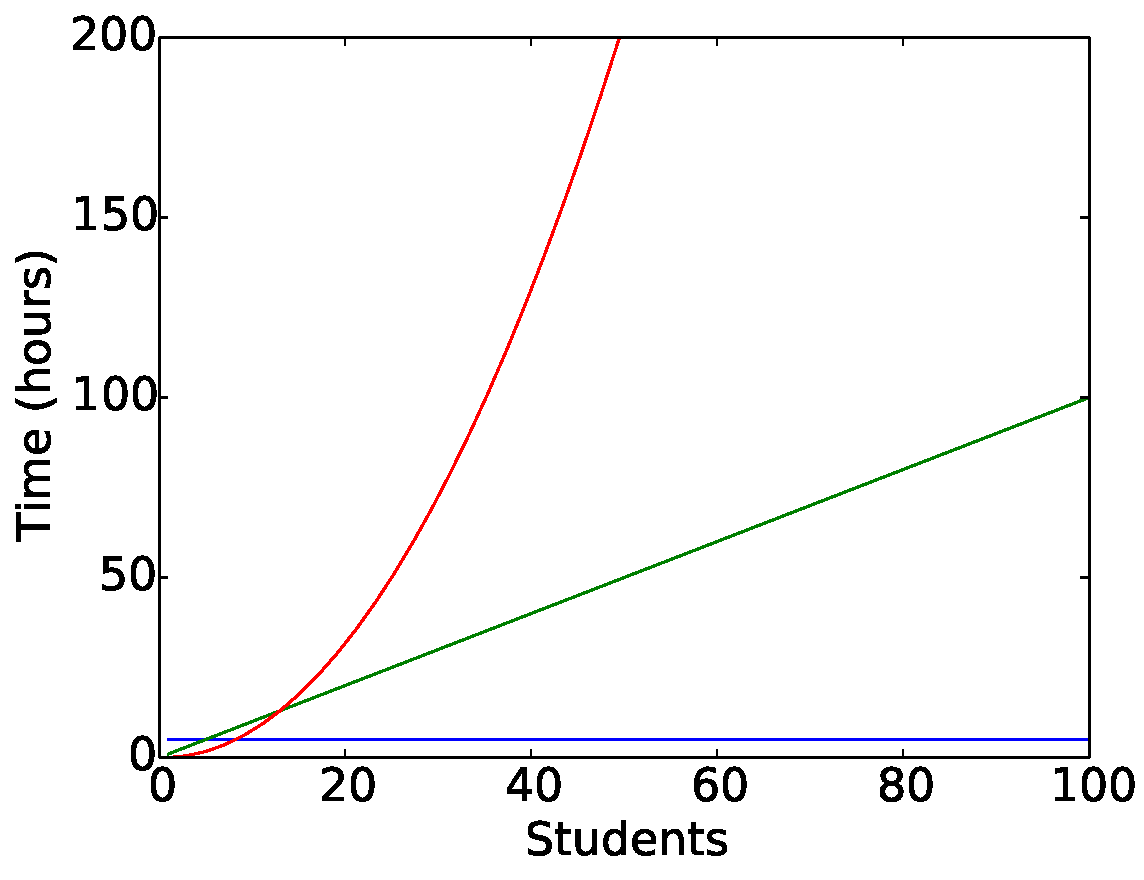
\includegraphics[width=\textwidth]{plot_all}
		\end{column}
		\begin{column}{0.47\textwidth}
			\begin{itemize}
				\item So if the number of students \textbf{doubles}... \pause
				\begin{itemize}
					\item The time it takes to mark the work \textbf{doubles} \pause
					\item The time it takes to weigh the work \textbf{stays the same} \pause
					\item The time it takes to check for plagiarism \textbf{quadruples}
				\end{itemize}
			\end{itemize}
		\end{column}
	\end{columns}
\end{frame}

\begin{frame}{Application}
	\begin{itemize}
		\item A game has $n$ objects on screen, and performs several operations in its main loop: \pause
			\begin{itemize}
				\item Reads player input \pause
				\item Updates each object \pause
				\item Checks for collisions between each pair of objects \pause
			\end{itemize}
		\item What is the time complexity of each of these operations?
		\item The designer wants to double the number of objects on screen.
			What will happen to the performance of the game?
	\end{itemize}
\end{frame}
